\documentclass{beamer}
%
% Choose how your presentation looks.
%
% For more themes, color themes and font themes, see:
% http://deic.uab.es/~iblanes/beamer_gallery/index_by_theme.html
%
%\mode<presentation>
%{
%  \usetheme{default}      % or try Darmstadt, Madrid, Warsaw, ...
%  \usecolortheme{default} % or try albatross, beaver, crane, ...
%  \usefonttheme{default}  % or try serif, structurebold, ...
%  \setbeamertemplate{navigation symbols}{}
%  \setbeamertemplate{caption}[numbered]
%} 

\usepackage[english]{babel}
\usepackage[utf8]{inputenc}
\usepackage[T1]{fontenc}
\usepackage{listings}
\usepackage{hyperref}

\title[Joint lab meeting]{Hands-on using NEMO: Simple batch job submission on BW-HPCs}
\author{Sina and Marieke at Joint Lab meeting}
\date{\today}

\begin{document}

\begin{frame}
  \titlepage
\end{frame}

\section{Background}

\begin{frame}{BW HPC Clusters}

\begin{itemize}
  \item BW-Cluster
  \begin{itemize}
      \item 24 GPU nodes
  \end{itemize}
  \item \href{https://wiki.bwhpc.de/e/NEMO/Hardware#Compute\_and\_Special\_Purpose\_Nodes}{Nemo}
  \begin{itemize}
      \item on \$HOME (permanent storage): 100GB 
      \item limited lifetime storage with workspaces: 10TB  
      \item One GPU node (nvidia)
  \end{itemize}
  \item Helix 
  \begin{itemize}
      \item > 50 GPUs (nvidia)
  \end{itemize}
\end{itemize}

\end{frame}

\section{Registration}


\begin{frame}{Registration for NEMO (or any other BW-HPC)}


\begin{enumerate}
    \item \href{https://wiki.bwhpc.de/e/Registration/bwUniCluster/Entitlement}{Check entitlement}

\end{enumerate}

\begin{figure}
    \centering
    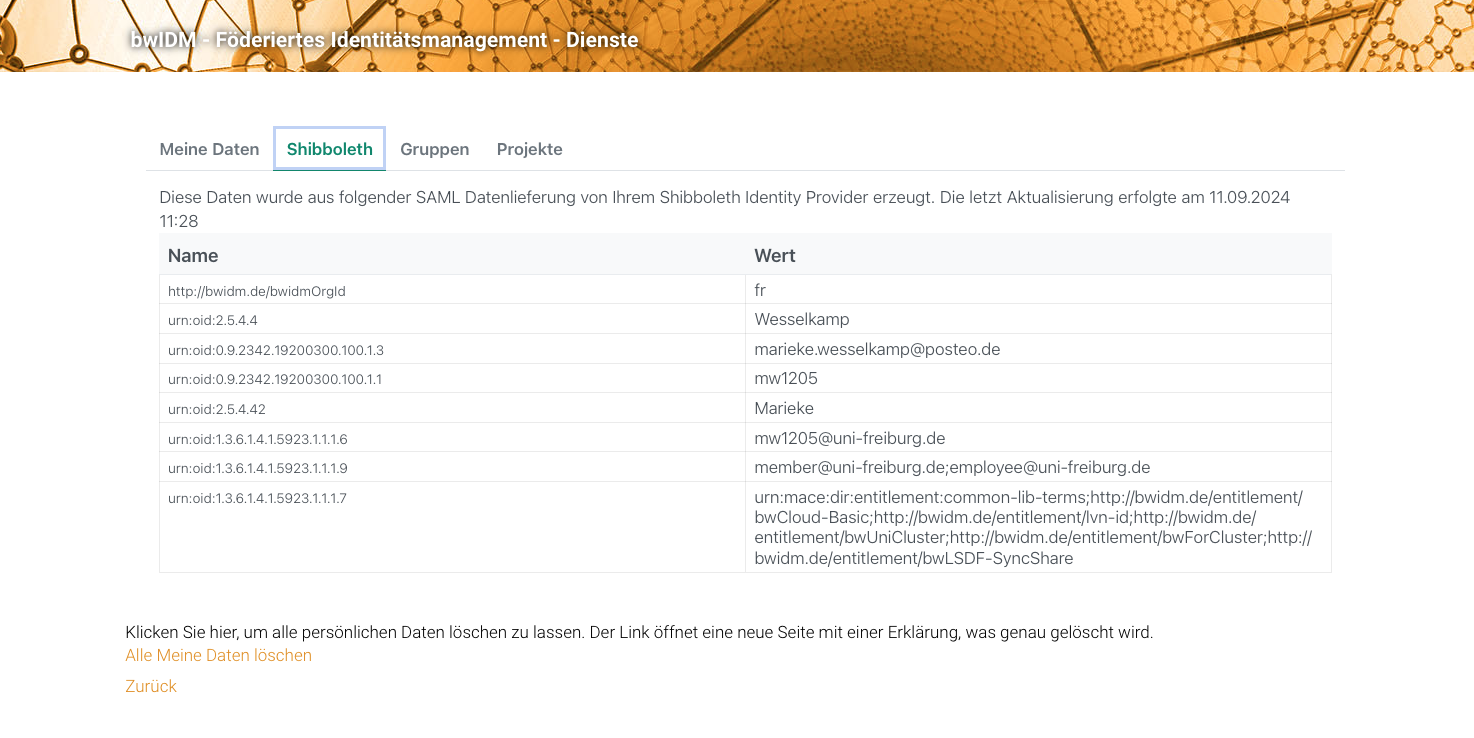
\includegraphics[width=0.95\linewidth]{figures/BWIDM_entitlement.png}
\end{figure}
Login with your Uni-Account to https://login.bwidm.de/

\end{frame}

\begin{frame}{Registration for NEMO}


\begin{enumerate}
    \item \href{https://wiki.bwhpc.de/e/Registration/bwUniCluster/Entitlement}{Check entitlement}
    \item \href{https://wiki.bwhpc.de/e/Registration/bwUniCluster/Service}{Register for cluster}
    \item \href{https://wiki.bwhpc.de/e/Registration/bwUniCluster/Questionnaire}{Fill in questionnaire within 14 days}
    
\end{enumerate}

\vspace{2cm}

\begin{columns}[onlytextwidth] 
  \begin{column}{0.5\textwidth}
      You will need to register 2 factor authentification, use for example OTP for generating one-time passowrds.
      \end{column}
    \hspace{0.02\textwidth} % add small horizontal space
    \begin{column}{0.5\textwidth}
      \begin{figure}
        \centering
        
\includegraphics[width=0.3\linewidth]{figures/OTP.png}
    \end{figure}
\end{column}
\end{columns}

  


\end{frame}


\section{Login}

\begin{frame}{Login to NEMO}

\begin{itemize}

\item \href{https://wiki.bwhpc.de/e/Registration/2FA}{Instructions on 2FA} 

\item \href{https://login.bwidm.de/}{For registering a new Token and setting a personalised password, see again: https://login.bwidm.de/}

\end{itemize}

\begin{figure}
    \centering
    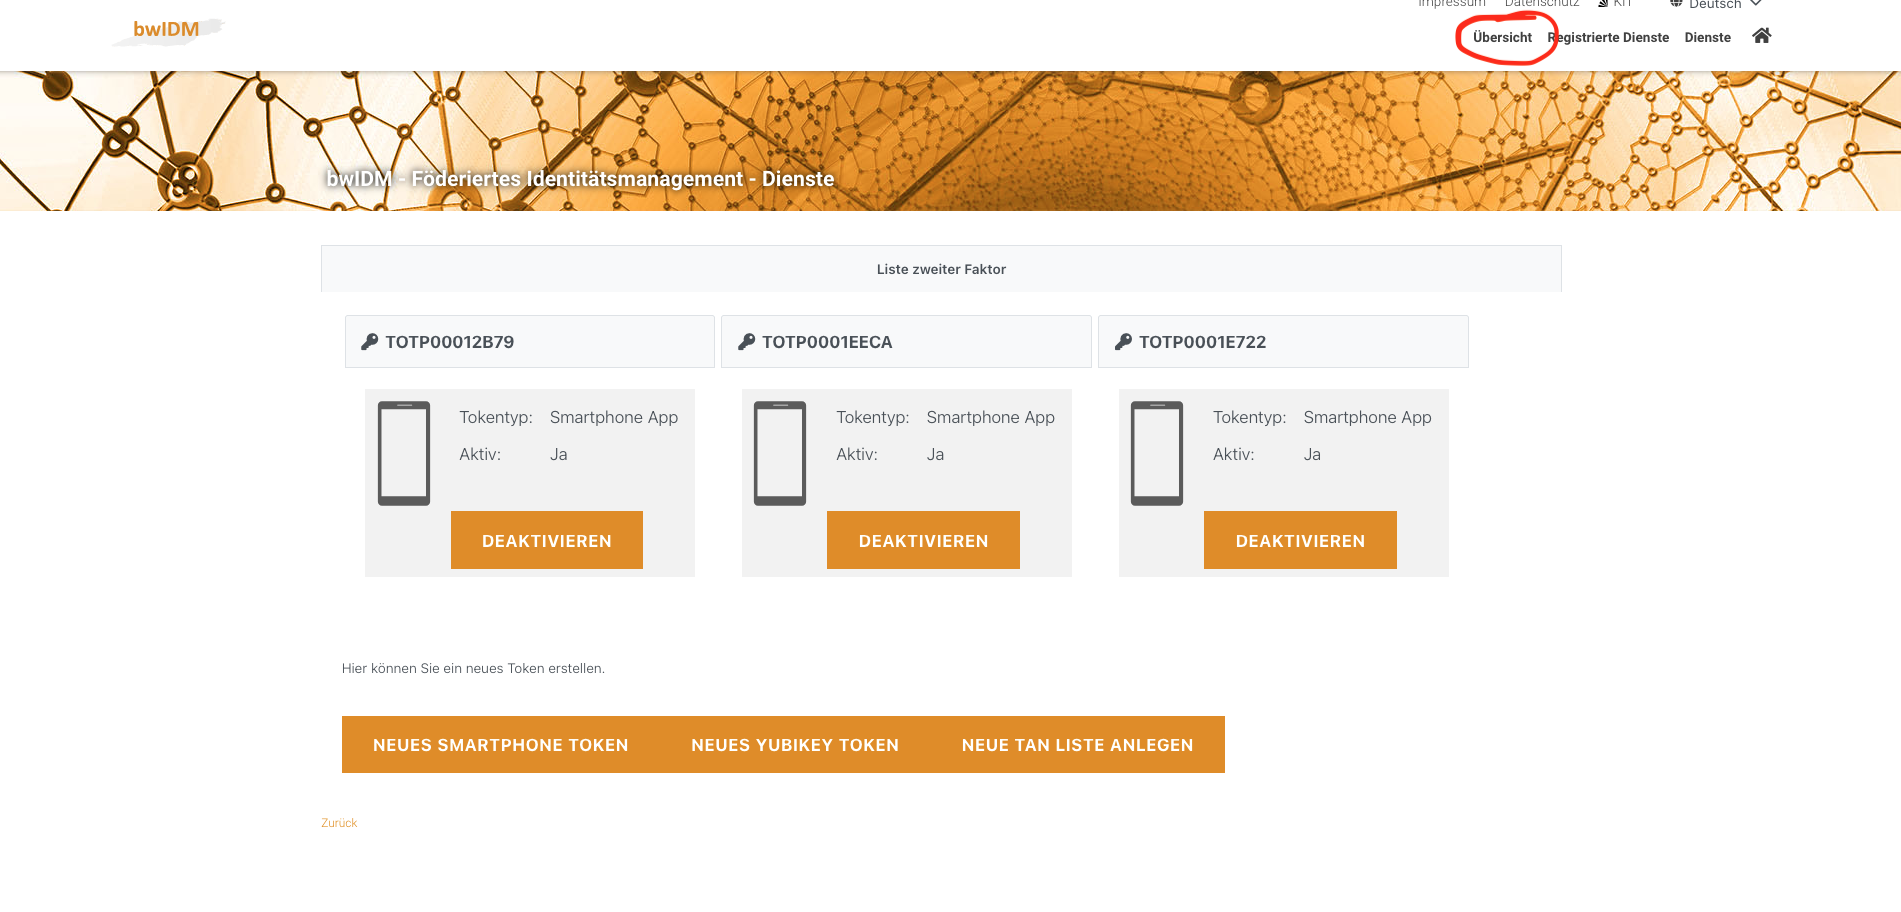
\includegraphics[width=0.95\linewidth]{figures/BWIDM.png}
\end{figure}

\end{frame}

\begin{frame}{Login to NEMO}

With a registered account \textbf{and from an eduroam network connection} (\href{https://www.rz.uni-freiburg.de/en/services/netztel-en/vpn-1?set_language=en}{Download VPN client}) you can access the HPC from your local shell with a secure shell client (SSH).

\begin{enumerate}
    \item Access cluster from your local shell: ssh fr\_mw1205@login1.nemo.uni-freiburg.de
    \item Create One Time Token on your mobile device
    \item Enter personalised password
\end{enumerate}
\vspace{0.6cm}
\scalebox{0.6}{
\lstinputlisting[]{output/output_1.txt}
}
\vspace{0.4cm}

If you prefer a graphical SSH client, use MobaXterm on Windows.

\end{frame}



\begin{frame}{Login node: Environment}

Navigation after successful login to Nemo: See you home directory and existing folders.

\scalebox{0.7}{
\lstinputlisting[]{output/output_3.txt}
}
\vspace{0.6cm}

\begin{itemize}
    \item Create new shell script: \texttt{touch example.sh}
    \item Create new directory: \texttt{mkdir example}
    \item Use a pre-installed texteditor (e.g.~vim) to access and modify files: \texttt{vi example.sh}
\end{itemize}


\end{frame}

\begin{frame}{Login Node Data Transfer}

\begin{itemize}
    \item Transfer a local file to the central cluster (and vice versa) using \texttt{scp} or \texttt{scp -r} from your local shell.
\end{itemize}

\vspace{0.5cm}

\begin{block}{Copy an entire folder from HPC to your local machine}
Run in your local terminal:
\vspace{0.1cm}
\footnotesize
\texttt{scp -r fr\_mw1205@login1.nemo.uni-freiburg.de:$\sim$/physics\_guided\_nn/results /Users/Marieke\_Wesselkamp/Projects/physics\_guided\_nn}
\end{block}
\vspace{0.1cm}

And vice versa for copying from local to HPC...

\end{frame}

\section{Job scripts}


\begin{frame}{Batch job specification}

Scheduling system on Nemo: MOAB. On Helix / BW-UniCluster: SLURM.

\begin{itemize}
    \item Job submission with shell script: example.sh
    \item Default directory at execution is working directory at submission: \texttt{pwd}
\end{itemize}

\end{frame}

\begin{frame}{Batch job specification}

\scalebox{0.5}{
\lstinputlisting[]{output/output_4.txt}
}

\end{frame}


\begin{frame}{Batch job specification}


\begin{itemize}
    \item Job submission with shell script: example.sh
    \item Default directory at execution is working directory at submission: \texttt{pwd}
    \item The maximum walltime for a job on Nemo is 96 hours (4 days). \textbf{Scales with requested ressources!}
    \item Nodes have 20 cores and 128 GB RAM. 
    \item If you request gpu: nodes=1:ppn=1:gpus=1 	
\end{itemize}


\end{frame}


\begin{frame}{Batch job specification: Computation environment}

\begin{itemize}
    \item WORKDIR = direction/to/your/project
    \item cd \$WORKDIR
    \item load conda: ml devel/conda
    \item activate your environment: conda activate your\_environment
    \item run script: python3 your\_file.py
    \item create environment from .yml file: conda env create -f environment.yml
\end{itemize}


\end{frame}

\section{Job submissions}

\begin{frame}{Batch job submission}

Specify queue 
\begin{itemize}
    \item Express for test runs: msub -q express ...
    \item GPU if you need it: msub -q gpu ... (32 cores with enabled simultaneous multithreading) 
\end{itemize}

See also : \href{https://wiki.bwhpc.de/e/NEMO/Moab}{https://wiki.bwhpc.de/e/NEMO/Moab}




\end{frame}

\begin{frame}{Batch job submission on Helix}

Hands on demonstration. For following the example, download shell script from: https://github.com/MWesselkamp/BW-HPC-Usage.


\end{frame}


\begin{frame}{Batch job submission on Helix}

\begin{figure}
    \centering
    
\includegraphics[width=0.85\linewidth]{examples/ScreenShots/S1.png}
\end{figure}

\end{frame}

\begin{frame}{Batch job submission on Helix}

\begin{figure}
    \centering
    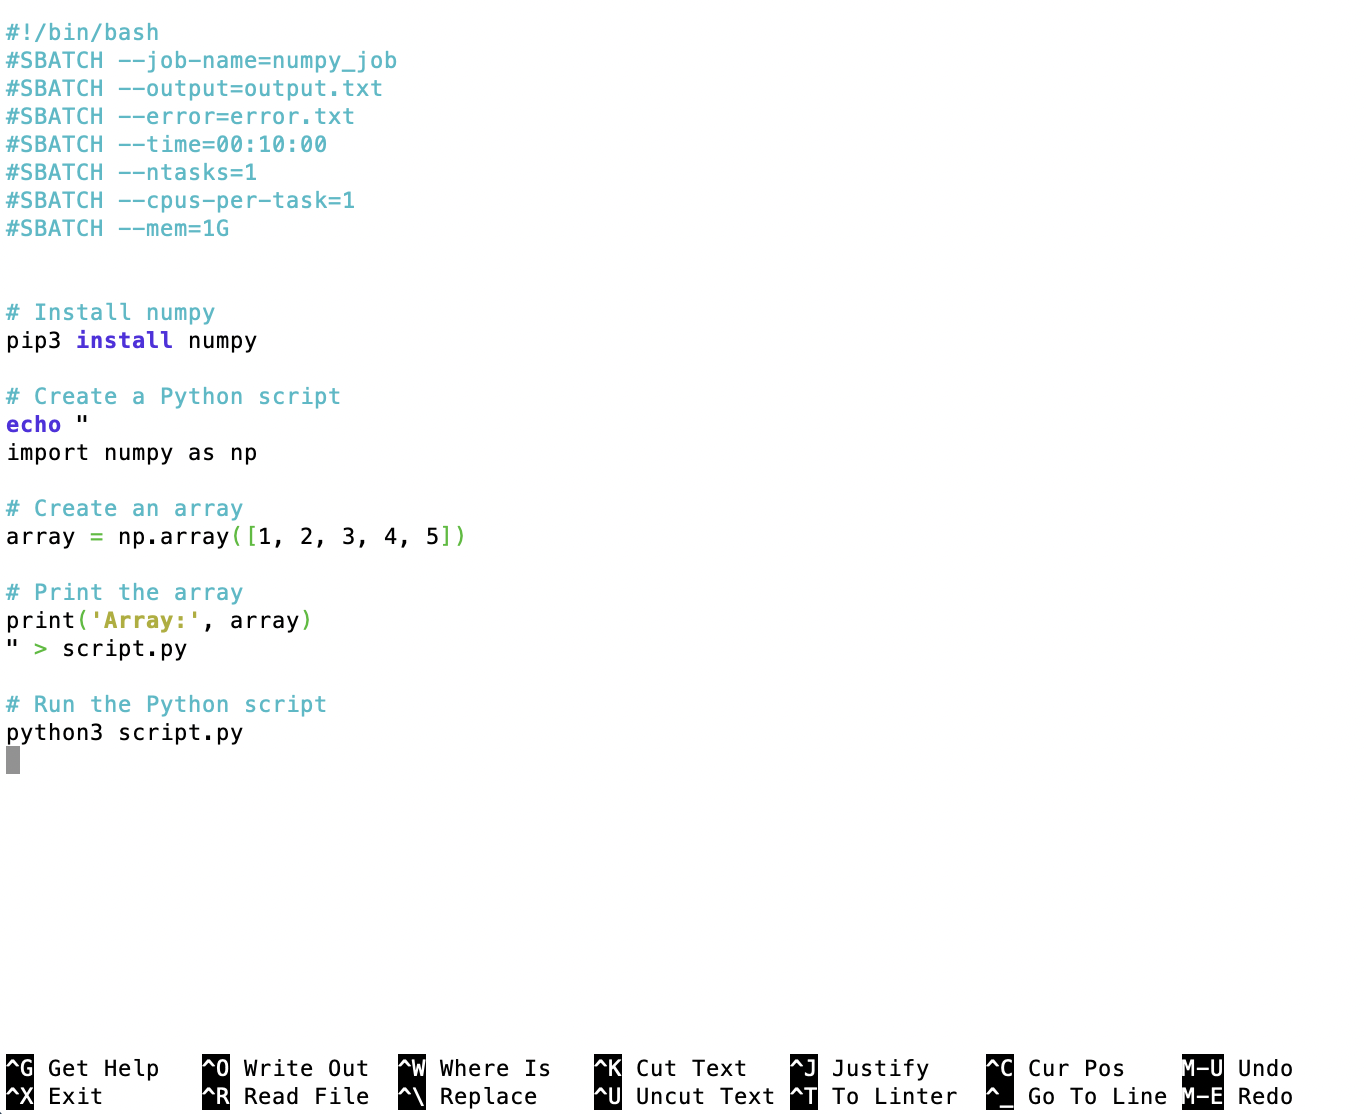
\includegraphics[width=0.85\linewidth]{examples/ScreenShots/S2.png}
\end{figure}

\end{frame}

\begin{frame}{Batch job submission on Helix}

After and during job execution, check output file for printed progress. 

\begin{figure}
    \centering
    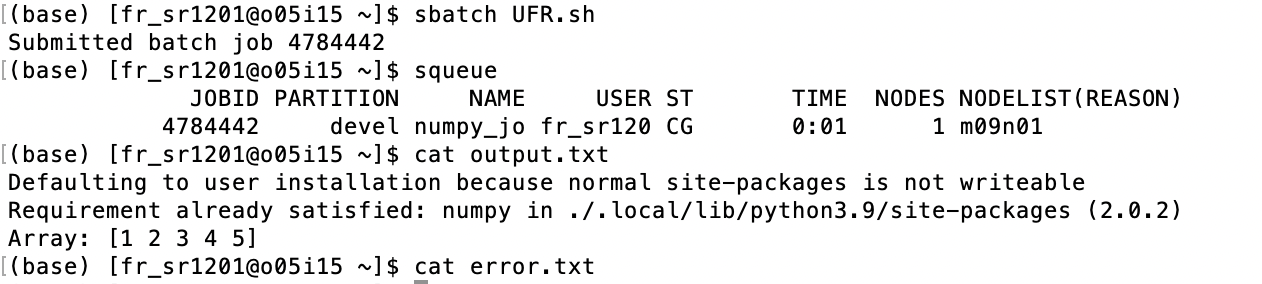
\includegraphics[width=1\linewidth]{examples/ScreenShots/S3.png}
\end{figure}

\end{frame}

\section{HPC cluster usage}

\begin{frame}{Job handling}

\begin{itemize}
    \item # Show my active jobs: \texttt{squeue} / \texttt{showq -u \$USER}
    \item # Cancel active jobs: \texttt{scancel jobID}
    \item # Monitor running job: \texttt{checkjob 12345}
\end{itemize}

\vspace{2cm}

Download slides at: https://github.com/MWesselkamp/BW-HPC-Usage.

\end{frame}


\end{document}
